%---------------------------------- Optimization frame -------------------------------
\begin{frame}{Global HPO workflow}
            \begin{figure}
                \centering
                \begin{tikzpicture}[node distance=1.5cm]

    % Define block styles
    \tikzstyle{class}=[rectangle split,rectangle split parts=2,draw,text centered]
    \tikzstyle{action} = [rectangle, rounded corners, minimum width=2cm, minimum height=0.8cm,text centered, draw=black, fill=red!30]
    \tikzstyle{decision} = [diamond,text centered, draw=black, fill=yellow!30]
    \tikzstyle{final} = [rectangle, minimum width=2cm, minimum height=1cm,text centered, draw=black]
    
    % Define arrow styles
    \tikzstyle{tarrow} = [thick,->,>=stealth]
    \tikzstyle{larrow} = [thick,dotted,->,>=stealth]
    \tikzstyle{coin} = [thick]
    \tikzstyle{light} = [thick,dotted]
    
    
    % Define nodes
    
    % black box function
    \node (model) [class, align=center]
        {
            \textbf{Model }
            \nodepart{second} Llama-3.2-1B \\ hyperparameters };  
    
    \node (trainer) [class, below of=model]
        {
            \textbf{Trainer}
            \nodepart{second} hyperparameters};
    
    \node (training)[action,right of = model,xshift=2cm]{Training};
    \node (evaluate)[action,below of = training]{Evaluate};
    
    \node(bbfunction)[draw, thick, dashed, rounded corners, fit=(model) (trainer) (training) (evaluate), inner sep=0.2cm, label=below:{Black-Box function}] {};
    
    
    %datasets
    \node (train_data) [class, right of=training,xshift=2cm]
        {
            \textbf{Training Dataset}
            \nodepart{second} Alpaca \cite{hashimoto_stanford_2024}};
    
    \node (val_data) [class, right of=evaluate,xshift=2cm]
        {
            \textbf{Validation/Testing Dataset}
            \nodepart{second} Hellaswag\cite{zellers_hellaswag_2019}, MMLU\cite{hendrycks_measuring_2021}};
    
    % decision
    \node (decision)[decision,below of = evaluate,yshift=-1cm,align=center]{if \\ $n_{eval} \leq n_{max}$ };
    
    \node (final)[final,right of = decision,xshift=2cm]{return best point};
    
    % HPO
    \node (hpo) [class, below of=trainer,yshift=-1cm]
        {
            \textbf{HPO}
            \nodepart{second} optimization loop};
    
    
    % functionnal node
    \node (trainerright) [right of=trainer]{};
    \node (modelright) [right of=model]{};
    \node (hpoleft) [left of = hpo]{};
    \node (modelleft) [left of = model]{};
    \node (trainerleft) [left of = trainer]{};
    
    
    % arrow inside bb function
    \draw [larrow] (model) -- (training);
    \draw [light] (trainer) -- (trainerright.center);
    \draw [light] (trainerright.center) -- (modelright.center);
    \draw [larrow] (modelright.center) -- (training);
    \draw [larrow] (training) -- (evaluate);
    
    % arrows outside bb function
    \draw [tarrow] (train_data) -- (training);
    \draw [tarrow] (val_data) -- (evaluate);
    \draw [tarrow] (evaluate) -- (decision);
    \draw [tarrow] (decision) -- (hpo);
    \draw [tarrow] (decision) -- (final);
    
    % arrow from hpo to bb function
    \draw [coin] (hpo) -- (hpoleft.center);
    \draw [coin] (hpoleft.center) -- (modelleft.center);
    \draw [tarrow] (modelleft.center) -- (model);
    \draw [tarrow] (trainerleft.center) -- (trainer);
    
    \end{tikzpicture}
                \caption{HPO workflow}
            \end{figure}
    
\end{frame}

%---------------------------------- Evaluation Function -------------------------------
\begin{frame}{Evaluate the solution}
    Use LitGPT framework with it's CLI to perform an evaluation of a solution. All models and datasets are taken from HuggingFace Hub.
    \begin{block}{Training}
        \begin{itemize}
            \item Model : Llama-3.2-1B
            \item dataset : Alpaca
            \item 1 epochs of training
            \item Fully Sharded Data Parallelism (FSDP) as distributed strategy
        \end{itemize}
    \end{block}

    \begin{block}{Evaluating}
        Based on lm\_eval library
        \begin{itemize}
            \item validation dataset : Hellaswag
            \item testing dataset : MMLU
        \end{itemize}
    \end{block}

    
\end{frame}

%---------------------------------- Optimization -------------------------------
\begin{frame}[allowframebreaks]{Optimization algorithms}

    \begin{columns}
        \begin{column}[b]{0.4\textwidth}
            \textbf{Partition Based Algorithm : Simultaneous Optimistic Optimization (SOO)}

            Perform a K-inary partition of the space, evaluating every center of partition during the expansion of a node.
            
        \end{column}        
        \begin{column}{0.6\textwidth}
            \begin{figure}[h]
                \centering
                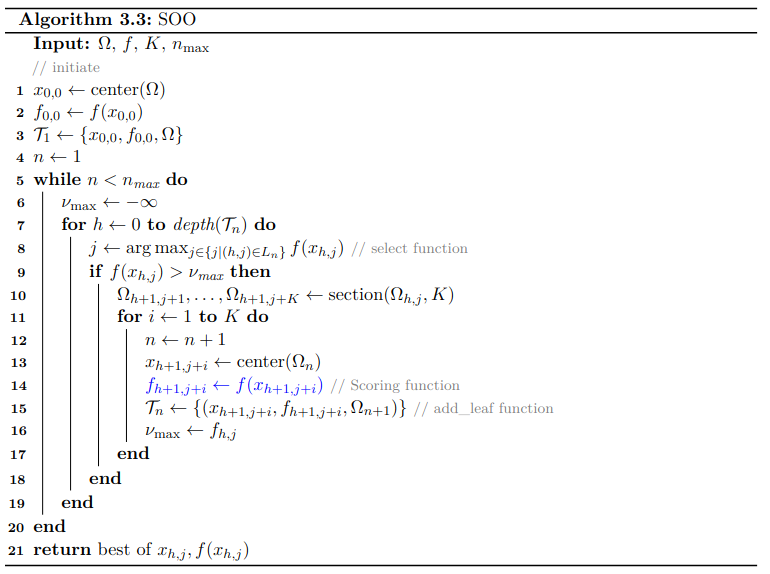
\includegraphics[trim={0 0 7cm 0},clip,height = 6.5cm]{imgs/algo/soo.png}
                \caption{SOO Algorithm}
            \end{figure}
        \end{column}
    \end{columns}

    \framebreak

    \begin{columns}
        \begin{column}{0.3\textwidth}
            \textbf{Surrogate Model Based Optimization : Bayesian Optimization with Gaussian Process (BO-GP)}

            Use Gaussian Process as a surrogate for the objective function, and optimize it to found the most promising point to evaluate
            
        \end{column}        
        \begin{column}{0.7\textwidth}
            \begin{figure}[h]
                \centering
                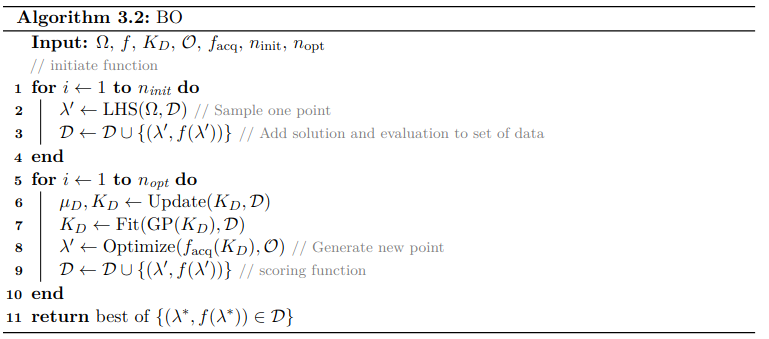
\includegraphics[height = 6cm]{imgs/algo/bo.png}
            \end{figure}
        \end{column}
    \end{columns}

    \framebreak

    \begin{columns}
        \begin{column}{0.5\textwidth}
            \textbf{Hybridation : Bayesian Multi-Scale Optimistic Optimization(BaMSOO)}

            Replace the scoring of SOO with a BO-GP based approximation to determine if it's relevant to evaluate the point.
            \begin{equation}
                \begin{split}
                \mathcal{UCB}(x| \mathcal D_t) = \mu(x|\mathcal D_t) +  B_N * \sigma(x|\mathcal D_t) 
                \\ \text{with } B_N = \sqrt{2 \log (\pi^2 N^2/6 \eta)} , \eta \in (0,1)      
                \end{split}  
                \label{eq:ucb}
            \end{equation}
            
        \end{column}        
        \begin{column}{0.5\textwidth}
            \begin{figure}[h]
                \centering
                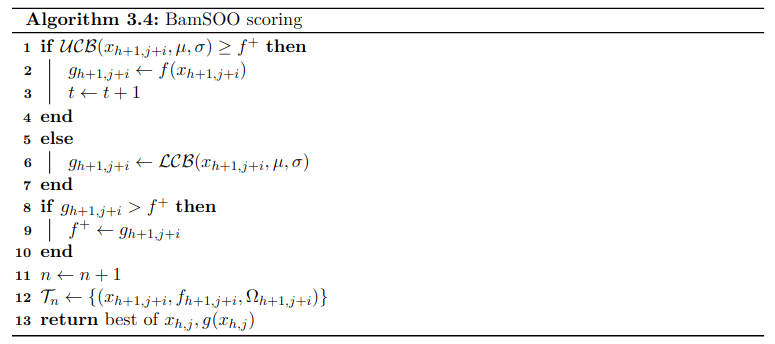
\includegraphics[trim={0 0 12cm 0},clip,height = 5cm]{imgs/algo/bamsoo_score.png}
            \end{figure}
        \end{column}
    \end{columns}

        
\end{frame}